\section{A PIM-oriented execution recommendation}
\label{sec:execution-sketch}
The measured mechanism is DRAM request scheduling and can matter to a CPU as well as to PIM. Its PIM relevance is a specific design decision: if a near-memory engine gathers vectors for HNSW distance evaluation, how should it expose the reads that are currently available? Moving computation closer to storage does not remove bank timing constraints. A placement that improves row reuse can still restrict useful overlap, and a frontend that interleaves chunks can help or hurt depending on the memory interface. This study establishes those conditional service effects, not an advantage unique to PIM.

\subsection{A concrete division of work and data}
Consider a host-controlled gather-and-distance design (Figure~\ref{fig:profile-execution}). Keep HNSW traversal, the visited set and the candidate/result queues on the host. Keep vectors and adjacency lists in memory addressable by a near-memory engine. The host reads a neighbour list, selects unvisited candidates and resolves their vector addresses. It sends a batch descriptor containing those addresses and original-order tags. A query vector is supplied once and retained near memory while that query runs. The engine gathers the batch, evaluates squared Euclidean distances and returns tagged distances; the host applies them in the original candidate order before choosing the next expansion.

This split is a proposed integration point, not an implemented platform. Vector gathering and per-candidate distance arithmetic are plausible near-memory operations because they consume resident arrays and return small results. Visited-set accesses, heap updates and graph control could also move to a programmable memory-side processor, but would require storage, synchronisation and a new execution evaluation. The present recommendation keeps them on the host to make that additional commitment explicit. Table~\ref{tab:pim-residency} summarises data residency and transfers.

\begin{table}[htbp]\centering\small
\caption[Data residency and transfers in the proposed PIM path]{One possible host-controlled gather-and-distance integration. Residency and transfers are design assumptions; only the recorded list and vector DRAM reads are timed by this thesis.}\label{tab:pim-residency}
\begin{tabular}{>{\raggedright\arraybackslash}p{0.22\textwidth}>{\raggedright\arraybackslash}p{0.31\textwidth}>{\raggedright\arraybackslash}p{0.36\textwidth}}
\toprule
Data & Proposed location & Movement or use\\\midrule
Vectors and adjacency & DRAM behind the near-memory engine & List IDs reach host control; candidate vectors feed local distance evaluation.\\
Query vector & Host and engine local storage & Send once per query per participating engine; reuse across candidate distances.\\
Visited set and search queues & Host & Updated after candidate discovery and ordered distance completion.\\
Node-to-slot mapping & Host in this example & Resolves IDs to vector addresses; mapping lookups are an additional cost.\\
Batch descriptors & Host to engine & Addresses, candidate identity/order tags and batch length.\\
Candidate data and results & Engine local storage & Buffer vector chunks or partial sums; return tagged distances to the host.\\\bottomrule
\end{tabular}
\end{table}

A gather-only engine that returns full vectors to host arithmetic still moves the vector payload across the host interface. Adding distance evaluation near memory is what could avoid that transfer. For a batch of $B$ candidates, the avoided payload would be $Bb$ bytes, replaced by descriptors and $B$ tagged distances, with query and neighbour-list transfers still required. This is byte accounting, not a bandwidth or energy result; protocol overhead, replication and repeated reads can alter total traffic. At 512 bytes the arithmetic uses the measured float32 representation. The hypothetical 128-byte experiment supplies no corresponding compressed-distance kernel or accuracy result.

\subsection{Dependencies and hardware requirements}
Candidate discovery must precede its vector requests. After a list arrives, reads for its available candidates can overlap, but the next graph expansion may depend on their distances. Request completion order must not change the order of search-state updates, stopping rules or ties. Reproducing distances also requires compatible numerical precision and reduction behaviour; preserving memory order alone cannot guarantee identical search on a different arithmetic unit. The following pseudocode expresses this dependency, with distance computation assigned to the engine and search updates to the host in the example above. It sketches the expansion stage; entry-vector evaluation and initial search-state setup are omitted.

\begin{lstlisting}
order = lookup_profile(configuration) or ORIGINAL
while search_needs_an_expansion():
    candidates = read_list_and_select_unvisited()
    for batch in consecutive_batches(candidates, B):
        addresses = resolve_vector_addresses(batch)
        chunks = make_native_reads(addresses, vector_bytes)
        for chunk in order_reads(chunks, order):
            submit_when_capacity_available(chunk)
        wait_for_batch_reads()
        for candidate in batch:  # original candidate order
            distance = compute_distance(candidate, query)
            update_search_state(candidate, distance)
\end{lstlisting}

Original order offers all chunks of one vector before offering the next vector's chunks; it does not wait for completion between vectors. Sorting orders the batch's chunk addresses. Round-robin offers chunk zero of every vector, then chunk one of every vector, and so on. A configuration profile selects between these established orders. Selection and fallback costs are discussed in Section~\ref{sec:profile-deployment}.

The target needs a programmable request frontend, several outstanding reads, completion tags, local storage for vectors or partial distances, query reuse and a distance unit with suitable arithmetic. To reproduce this study's intervention, it must expose ordering at the modelled 32-byte granularity and a compatible address mapping. A DMA interface that only accepts whole-vector transfers may hide that choice. A bank-local processor may also lack access to the cross-bank pool used by this single-channel experiment: partitioning, routing and query distribution would then need separate measurement. The assumed interface is not a claim about commercial UPMEM or every HBM-based PIM design~\cite{primer,upanns}.

This is an illustrative implementation sketch, not the measured program. The replay supplies the recorded candidates and addresses in advance and times their DRAM service. It does not execute candidate selection, address resolution, arithmetic, visited-state updates, result queues or local-buffer accesses. Those operations must be charged in a target implementation, along with any host/PIM transfers. Small-batch replay also adds drains without simulating the computation between them.

\begin{figure}[htbp]\centering
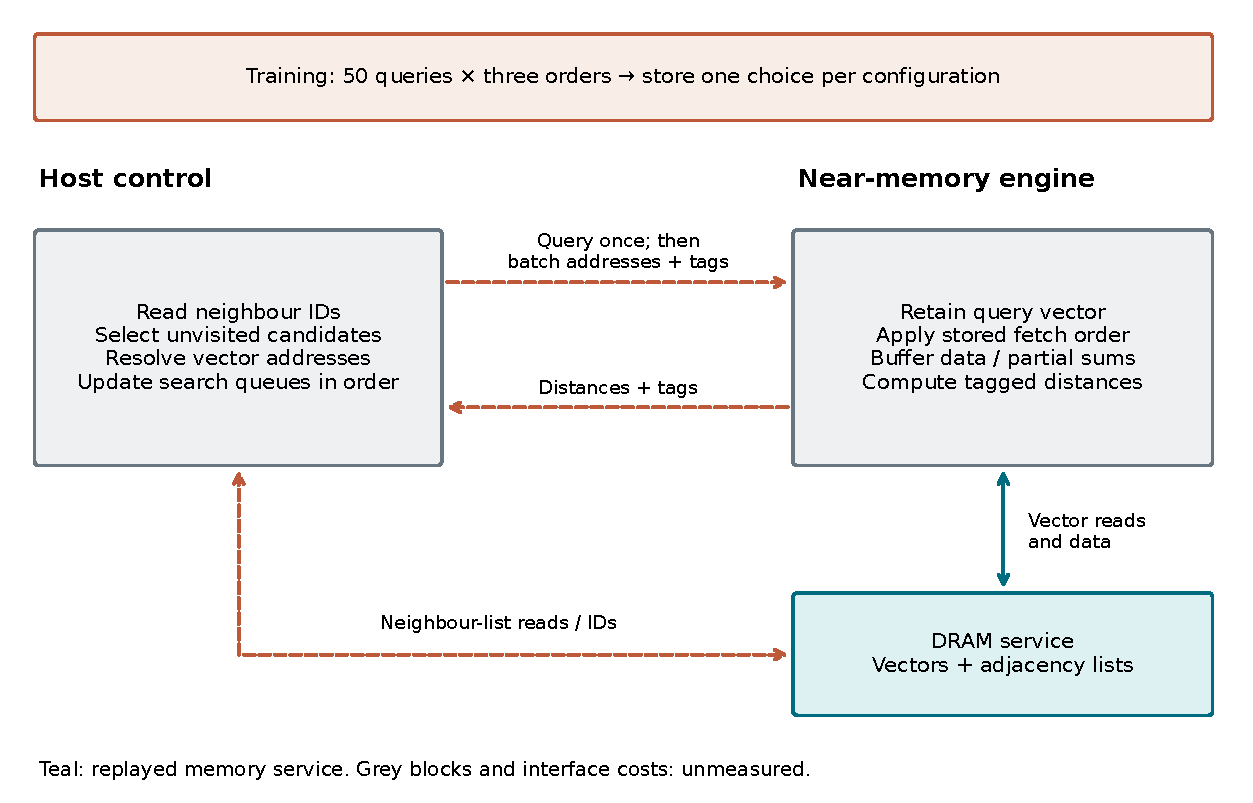
\includegraphics[width=\textwidth]{generated/profiled_fetch_execution.pdf}
\caption[Proposed host and near-memory execution boundary]{A host-controlled gather-and-distance design to evaluate. Training selects an order per configuration. Dashed arrows cross the host/engine boundary; the query is retained for reuse. Teal identifies the DRAM service included in replay, including neighbour-list reads. Grey control and computation blocks and all interface costs remain unmeasured. Returning distances instead of vectors requires the proposed distance unit.}\label{fig:profile-execution}
\end{figure}

For a straightforward full-vector buffer, $B$ candidates of $b$ bytes require at most $Bb$ payload bytes, plus addresses, query data and search state. At 512 bytes, batches of two and eight require 1 and 4 KiB respectively. A full 32-candidate base-layer list would require 16 KiB. These are storage calculations for this example; they are not measured scratch-memory traffic or a minimum for every design. A streaming distance kernel could use a different buffering strategy and would need its own evaluation.

\subsection{What the service result contributes to this design}
The measured saving supplies a target to test against: the default 512-byte BFS round-robin comparison leaves approximately \RoundRobinBFSSavedFloat{} simulated service cycles per query before extra costs. It compares two request orders inside the same memory model, not host execution with PIM execution. A host round trip at each expansion could dominate this saving. Conversely, keeping traversal near memory would change control and communication costs and possibly the available request overlap. Concurrent queries may already supply bank diversity, reducing the value of reordering one query. These possibilities explain why the service result guides an implementation experiment without predicting its application outcome.

For a complete accelerator, the next directly related experiment would implement this gather boundary with the target's native transfer granularity and local storage, then compare original, sorted and round-robin execution at the same recall and concurrency. Include a host-only HNSW baseline, the same accelerator with original-order fetch, and the profiled path with calibration cost reported separately. Measure end-to-end query latency and throughput, local-buffer occupancy, communication and distance-computation time. These controls would distinguish a scheduling benefit from an accelerator or batching benefit. The present evidence helps choose this experiment; it does not supply its unmeasured outcome.
